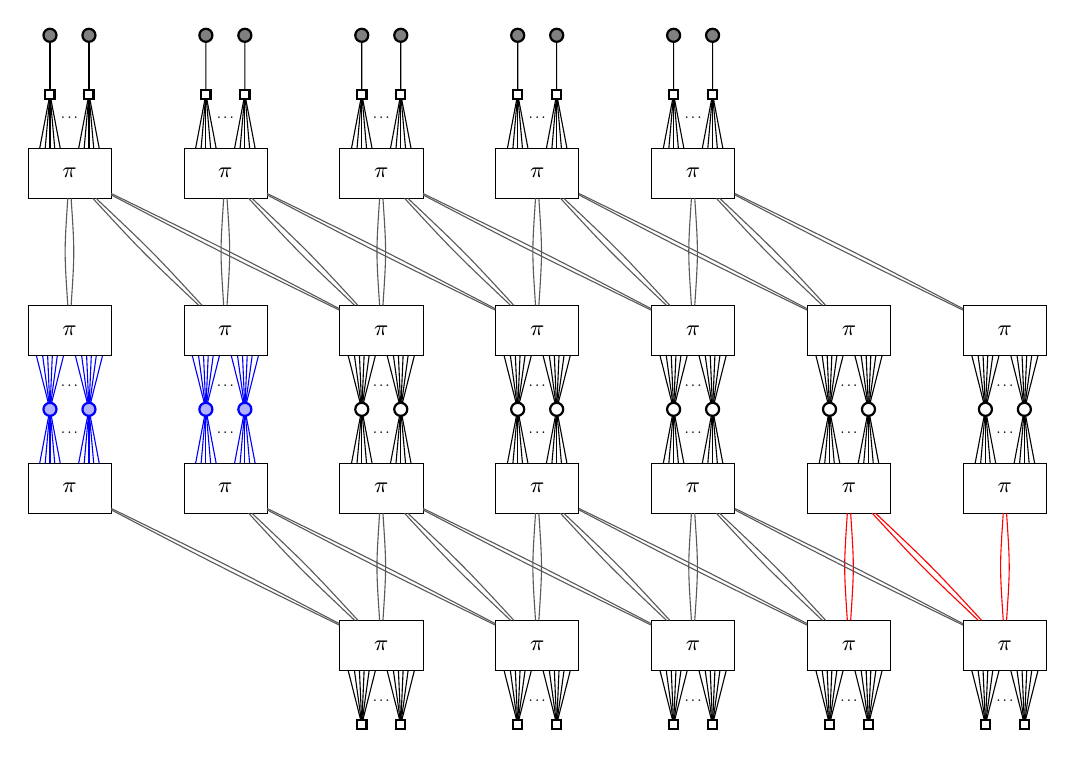
\begin{tikzpicture}[  xscale=0.33,yscale=1]
  \def \nodescale {0.5}
  \tikzset{  
  bitnode/.style={circle, scale=\nodescale, minimum size=4pt,thick,draw=black,fill=white},
  bitnodeblack/.style={circle,scale=\nodescale, minimum size=10pt,thick,draw=black,fill=white},
  bitnodewhite/.style={circle,scale=\nodescale,minimum size=10pt,thick,draw=white,fill=white},
  bitnode2/.style={circle,scale=\nodescale,minimum size=4pt,thick,draw=black,fill=gray},
  bitnode2black/.style={circle,scale=\nodescale,minimum size=2pt,thick,draw=black,fill=gray},
  bitnode2white/.style={circle,scale=\nodescale,minimum size=2pt,thick,draw=white,fill=white},
  checknode/.style={rectangle,scale=\nodescale,minimum width=2pt,minimum height =2pt,thick,draw=black,fill=white},
  checknodeblack/.style={rectangle, scale=\nodescale, minimum size=2pt,thick,draw=black,fill=white},
  checknodewhite/.style={rectangle, scale=\nodescale, minimum size=2pt,thick,draw=white,fill=white},
  permnode/.style={rectangle,very thin,minimum width=30pt,minimum height=18pt,fill=white,draw=black},
  permnodeblack/.style={rectangle,very thin,minimum width=30pt,minimum height=18pt,fill=white,draw=black},
  permnodewhite/.style={rectangle,very thin,minimum width=30pt,minimum height=18pt,fill=white,draw=white},
  permedge/.style={black!65},
  permedgeblack/.style={black!65},
  permedgewhite/.style={white}
  }
  
  \def \cndist {0.75}
  \def \vndist {0.75}
  \def \ccndist {0.75}
  \def \vvny {2.75}
  \def \cny {2}
  \def \vny {-2}
  \def \ccny {-6}

  \def \midx   {0.5}


    \foreach \x/\i/\ldgcol/\ldpcol in {0/1/black/white,6/2/black/white} {
      \draw[\ldgcol] (\x-\cndist, \cny) +(0,0) -- +(240:1);
      \draw[\ldgcol] (\x-\cndist, \cny) +(0,0) -- +(255:1);
      \draw[\ldgcol] (\x-\cndist, \cny) +(0,0) -- +(270:1);
      \draw[\ldgcol] (\x-\cndist, \cny) +(0,0) -- +(285:1);
      \draw[\ldgcol] (\x-\cndist, \cny) +(0,0) -- +(300:1);

      \draw[\ldgcol] (\x+\cndist, \cny) +(0,0) -- +(240:1);
      \draw[\ldgcol] (\x+\cndist, \cny) +(0,0) -- +(255:1);
      \draw[\ldgcol] (\x+\cndist, \cny) +(0,0) -- +(270:1);
      \draw[\ldgcol] (\x+\cndist, \cny) +(0,0) -- +(285:1);
      \draw[\ldgcol] (\x+\cndist, \cny) +(0,0) -- +(300:1);

      \draw[blue] (\x-\vndist, \vny) +(0,0) -- +(52.5:1);
      \draw[blue] (\x-\vndist, \vny) +(0,0) -- +(67.5:1);
      \draw[blue] (\x-\vndist, \vny) +(0,0) -- +(82.5:1);
      \draw[blue] (\x-\vndist, \vny) +(0,0) -- +(97.5:1);
      \draw[blue] (\x-\vndist, \vny) +(0,0) -- +(112.5:1);
      \draw[blue] (\x-\vndist, \vny) +(0,0) -- +(127.5:1);

      \draw[blue] (\x+\vndist, \vny) +(0,0) -- +(52.5:1);
      \draw[blue] (\x+\vndist, \vny) +(0,0) -- +(67.5:1);
      \draw[blue] (\x+\vndist, \vny) +(0,0) -- +(82.5:1);
      \draw[blue] (\x+\vndist, \vny) +(0,0) -- +(97.5:1);
      \draw[blue] (\x+\vndist, \vny) +(0,0) -- +(112.5:1);
      \draw[blue] (\x+\vndist, \vny) +(0,0) -- +(127.5:1);

      \draw[blue] (\x-\vndist, \vny) +(0,0) -- +(240:1);
      \draw[blue] (\x-\vndist, \vny) +(0,0) -- +(255:1);
      \draw[blue] (\x-\vndist, \vny) +(0,0) -- +(270:1);
      \draw[blue] (\x-\vndist, \vny) +(0,0) -- +(285:1);
      \draw[blue] (\x-\vndist, \vny) +(0,0) -- +(300:1);

      \draw[blue] (\x+\vndist, \vny) +(0,0) -- +(240:1);
      \draw[blue] (\x+\vndist, \vny) +(0,0) -- +(255:1);
      \draw[blue] (\x+\vndist, \vny) +(0,0) -- +(270:1);
      \draw[blue] (\x+\vndist, \vny) +(0,0) -- +(285:1);
      \draw[blue] (\x+\vndist, \vny) +(0,0) -- +(300:1);

      \draw[\ldpcol] (\x-\vndist, \ccny) +(0,0) -- +(52.5:1);
      \draw[\ldpcol] (\x-\vndist, \ccny) +(0,0) -- +(67.5:1);
      \draw[\ldpcol] (\x-\vndist, \ccny) +(0,0) -- +(82.5:1);
      \draw[\ldpcol] (\x-\vndist, \ccny) +(0,0) -- +(97.5:1);
      \draw[\ldpcol] (\x-\vndist, \ccny) +(0,0) -- +(112.5:1);
      \draw[\ldpcol] (\x-\vndist, \ccny) +(0,0) -- +(127.5:1);

      \draw[\ldpcol] (\x+\vndist, \ccny) +(0,0) -- +(52.5:1);
      \draw[\ldpcol] (\x+\vndist, \ccny) +(0,0) -- +(67.5:1);
      \draw[\ldpcol] (\x+\vndist, \ccny) +(0,0) -- +(82.5:1);
      \draw[\ldpcol] (\x+\vndist, \ccny) +(0,0) -- +(97.5:1);
      \draw[\ldpcol] (\x+\vndist, \ccny) +(0,0) -- +(112.5:1);
      \draw[\ldpcol] (\x+\vndist, \ccny) +(0,0) -- +(127.5:1);

      \node[checknode\ldgcol] (c1\i) at (\x-\cndist, \cny) {};
      \node[checknode\ldgcol] (c2\i) at (\x+\cndist, \cny) {};
      \node[circle,thick,draw=blue,fill=blue!30, scale=0.5] (v1\i) at (\x-\vndist, \vny) {};
      \node[circle,thick,draw=blue,fill=blue!30, scale=0.5] (v2\i) at (\x+\vndist, \vny) {};
      \node[checknode\ldpcol] (cc1\i) at (\x-\ccndist, \ccny) {};
      \node[checknode\ldpcol] (cc2\i) at (\x+\ccndist, \ccny) {};

      \node[bitnode2\ldgcol] (vv1\i) at (\x-\cndist,\vvny) {};
      \node[bitnode2\ldgcol] (vv2\i) at (\x+\cndist,\vvny) {};
      \draw[\ldgcol] (vv1\i) -- (c1\i);
      \draw[\ldgcol] (vv2\i) -- (c2\i);

      \node[\ldpcol] at (\x,-5.7) {\tiny{$...$}};
      \node at (\x,-2.3) {\tiny{$...$}};
      \node at (\x,-1.7) {\tiny{$...$}};
      \node[\ldgcol] at (\x,1.7) {\tiny{$...$}};
      
      \node[permnode\ldgcol] (perm1_node\i) at (\x,\cny-1) {\textcolor{\ldgcol}{\footnotesize{$\pi$}}};
      \node[permnode] (perm2_node\i) at (\x,\vny+1) {\footnotesize{$\pi$}};
      \node[permnode] (perm3_node\i) at (\x,\vny-1) {\footnotesize{$\pi$}};
      \node[permnode\ldpcol] (perm4_node\i) at (\x,\ccny+1) {\textcolor{\ldpcol}{\footnotesize{$\pi$}}};
    }

    \foreach \x/\i/\ldgcol/\ldpcol in {12/3/black/black,18/4/black/black,24/5/black/black,30/6/white/black,36/7/white/black} {
      \draw[\ldgcol] (\x-\cndist, \cny) +(0,0) -- +(240:1);
      \draw[\ldgcol] (\x-\cndist, \cny) +(0,0) -- +(255:1);
      \draw[\ldgcol] (\x-\cndist, \cny) +(0,0) -- +(270:1);
      \draw[\ldgcol] (\x-\cndist, \cny) +(0,0) -- +(285:1);
      \draw[\ldgcol] (\x-\cndist, \cny) +(0,0) -- +(300:1);

      \draw[\ldgcol] (\x+\cndist, \cny) +(0,0) -- +(240:1);
      \draw[\ldgcol] (\x+\cndist, \cny) +(0,0) -- +(255:1);
      \draw[\ldgcol] (\x+\cndist, \cny) +(0,0) -- +(270:1);
      \draw[\ldgcol] (\x+\cndist, \cny) +(0,0) -- +(285:1);
      \draw[\ldgcol] (\x+\cndist, \cny) +(0,0) -- +(300:1);

      \draw[] (\x-\vndist, \vny) +(0,0) -- +(52.5:1);
      \draw[] (\x-\vndist, \vny) +(0,0) -- +(67.5:1);
      \draw[] (\x-\vndist, \vny) +(0,0) -- +(82.5:1);
      \draw[] (\x-\vndist, \vny) +(0,0) -- +(97.5:1);
      \draw[] (\x-\vndist, \vny) +(0,0) -- +(112.5:1);
      \draw[] (\x-\vndist, \vny) +(0,0) -- +(127.5:1);

      \draw[] (\x+\vndist, \vny) +(0,0) -- +(52.5:1);
      \draw[] (\x+\vndist, \vny) +(0,0) -- +(67.5:1);
      \draw[] (\x+\vndist, \vny) +(0,0) -- +(82.5:1);
      \draw[] (\x+\vndist, \vny) +(0,0) -- +(97.5:1);
      \draw[] (\x+\vndist, \vny) +(0,0) -- +(112.5:1);
      \draw[] (\x+\vndist, \vny) +(0,0) -- +(127.5:1);

      \draw[] (\x-\vndist, \vny) +(0,0) -- +(240:1);
      \draw[] (\x-\vndist, \vny) +(0,0) -- +(255:1);
      \draw[] (\x-\vndist, \vny) +(0,0) -- +(270:1);
      \draw[] (\x-\vndist, \vny) +(0,0) -- +(285:1);
      \draw[] (\x-\vndist, \vny) +(0,0) -- +(300:1);

      \draw[] (\x+\vndist, \vny) +(0,0) -- +(240:1);
      \draw[] (\x+\vndist, \vny) +(0,0) -- +(255:1);
      \draw[] (\x+\vndist, \vny) +(0,0) -- +(270:1);
      \draw[] (\x+\vndist, \vny) +(0,0) -- +(285:1);
      \draw[] (\x+\vndist, \vny) +(0,0) -- +(300:1);

      \draw[\ldpcol] (\x-\vndist, \ccny) +(0,0) -- +(52.5:1);
      \draw[\ldpcol] (\x-\vndist, \ccny) +(0,0) -- +(67.5:1);
      \draw[\ldpcol] (\x-\vndist, \ccny) +(0,0) -- +(82.5:1);
      \draw[\ldpcol] (\x-\vndist, \ccny) +(0,0) -- +(97.5:1);
      \draw[\ldpcol] (\x-\vndist, \ccny) +(0,0) -- +(112.5:1);
      \draw[\ldpcol] (\x-\vndist, \ccny) +(0,0) -- +(127.5:1);

      \draw[\ldpcol] (\x+\vndist, \ccny) +(0,0) -- +(52.5:1);
      \draw[\ldpcol] (\x+\vndist, \ccny) +(0,0) -- +(67.5:1);
      \draw[\ldpcol] (\x+\vndist, \ccny) +(0,0) -- +(82.5:1);
      \draw[\ldpcol] (\x+\vndist, \ccny) +(0,0) -- +(97.5:1);
      \draw[\ldpcol] (\x+\vndist, \ccny) +(0,0) -- +(112.5:1);
      \draw[\ldpcol] (\x+\vndist, \ccny) +(0,0) -- +(127.5:1);

      \node[checknode\ldgcol] (c1\i) at (\x-\cndist, \cny) {};
      \node[checknode\ldgcol] (c2\i) at (\x+\cndist, \cny) {};
      \node[bitnode] (v1\i) at (\x-\vndist, \vny) {};
      \node[bitnode] (v2\i) at (\x+\vndist, \vny) {};
      \node[checknode\ldpcol] (cc1\i) at (\x-\ccndist, \ccny) {};
      \node[checknode\ldpcol] (cc2\i) at (\x+\ccndist, \ccny) {};

      \node[bitnode2\ldgcol] (vv1\i) at (\x-\cndist,\vvny) {};
      \node[bitnode2\ldgcol] (vv2\i) at (\x+\cndist,\vvny) {};
      \draw[\ldgcol] (vv1\i) -- (c1\i);
      \draw[\ldgcol] (vv2\i) -- (c2\i);

      \node[\ldpcol] at (\x,-5.7) {\tiny{$...$}};
      \node at (\x,-2.3) {\tiny{$...$}};
      \node at (\x,-1.7) {\tiny{$...$}};
      \node[\ldgcol] at (\x,1.7) {\tiny{$...$}};
      
      \node[permnode\ldgcol] (perm1_node\i) at (\x,\cny-1) {\textcolor{\ldgcol}{\footnotesize{$\pi$}}};
      \node[permnode] (perm2_node\i) at (\x,\vny+1) {\footnotesize{$\pi$}};
      \node[permnode] (perm3_node\i) at (\x,\vny-1) {\footnotesize{$\pi$}};
      \node[permnode\ldpcol] (perm4_node\i) at (\x,\ccny+1) {\textcolor{\ldpcol}{\footnotesize{$\pi$}}};
    }

    % \draw[permedge] (perm1_node\i) .. controls (\x-0.2,0) .. (perm2_node\i);
    % \draw[permedge] (perm1_node\i) .. controls (\x+0.2,0) .. (perm2_node\i);
    % \draw[permedge] (perm3_node\i) .. controls (\x-0.2,-4) .. (perm4_node\i);
    % \draw[permedge] (perm3_node\i) .. controls (\x+0.2,-4) .. (perm4_node\i);

    % 0/1,6/2,12/3,18/4,24/5,30/6,36/7

    \foreach \x/\i in {0/1,6/2,12/3,18/4,24/5} {
      \draw[permedge] (perm1_node\i) .. controls (\x-0.2,0) .. (perm2_node\i);
      \draw[permedge] (perm1_node\i) .. controls (\x+0.2,0) .. (perm2_node\i);
    }

    \foreach \x/\i/\xn/\in in {0/1/6/2,6/2/12/3,12/3/18/4,18/4/24/5,24/5/30/6} {
      \draw[permedge] (perm1_node\i) .. controls (0.5*\x+0.5*\xn-0.2,0) .. (perm2_node\in);
      \draw[permedge] (perm1_node\i) .. controls (0.5*\x+0.5*\xn+0.2,0) .. (perm2_node\in);
    }

    \foreach \x/\i/\xn/\in in {0/1/12/3,6/2/18/4,12/3/24/5,18/4/30/6,24/5/36/7} {
      \draw[permedge] (perm1_node\i) .. controls (0.5*\x+0.5*\xn-0.2,0) .. (perm2_node\in);
      \draw[permedge] (perm1_node\i) .. controls (0.5*\x+0.5*\xn+0.2,0) .. (perm2_node\in);
    }

    \foreach \x/\i in {12/3,18/4,24/5} {
      \draw[permedge] (perm3_node\i) .. controls (\x-0.2,-4) .. (perm4_node\i);
      \draw[permedge] (perm3_node\i) .. controls (\x+0.2,-4) .. (perm4_node\i);
    }

    \foreach \x/\i in {30/6,36/7} {
      \draw[red] (perm3_node\i) .. controls (\x-0.2,-4) .. (perm4_node\i);
      \draw[red] (perm3_node\i) .. controls (\x+0.2,-4) .. (perm4_node\i);
    }

    \foreach \x/\i/\xn/\in in {12/3/6/2,18/4/12/3,24/5/18/4,30/6/24/5} {
      \draw[permedge] (perm3_node\in) .. controls (0.5*\x+0.5*\xn-0.2,-4) .. (perm4_node\i);
      \draw[permedge] (perm3_node\in) .. controls (0.5*\x+0.5*\xn+0.2,-4) .. (perm4_node\i);
    }

    \foreach \x/\i/\xn/\in in {36/7/30/6} {
      \draw[red] (perm3_node\in) .. controls (0.5*\x+0.5*\xn-0.2,-4) .. (perm4_node\i);
      \draw[red] (perm3_node\in) .. controls (0.5*\x+0.5*\xn+0.2,-4) .. (perm4_node\i);
    }

    \foreach \x/\i/\xn/\in in {12/3/0/1,18/4/6/2,24/5/12/3,30/6/18/4,36/7/24/5} {
      \draw[permedge] (perm3_node\in) .. controls (0.5*\x+0.5*\xn-0.2,-4) .. (perm4_node\i);
      \draw[permedge] (perm3_node\in) .. controls (0.5*\x+0.5*\xn+0.2,-4) .. (perm4_node\i);
    }

  
\end{tikzpicture}



%%% Local Variables: 
%%% mode: latex
%%% TeX-master: "../talk"
%%% End: 
